\clearpage

\section{Fork}

\begin{tcolorbox}	
\begin{tabular}{p{2.75cm} p{0.2cm} p{10.5cm}} 	
\textbf{Header File}   &:& fork.h \\
\textbf{Source File}   &:& fork.cpp \\
\textbf{Version}       &:& 201711119 (Responsible: Romil Patel)
\end{tabular}
\end{tcolorbox}

\subsection*{Input Parameters}

---- NA ----

\subsection*{Input Signals}

\textbf{Number}: 1

\textbf{Type}: t\_real (TimeContinuousAmplitudeContinuousReal)

\subsection*{Output Signals}

\textbf{Number}: 2

\textbf{Type}: t\_real (TimeContinuousAmplitudeContinuousReal)

\subsection*{Functional Description}

This block accepts a time domain signal and outputs two replicas of the input signal.

\begin{figure}[h]
	\centering
	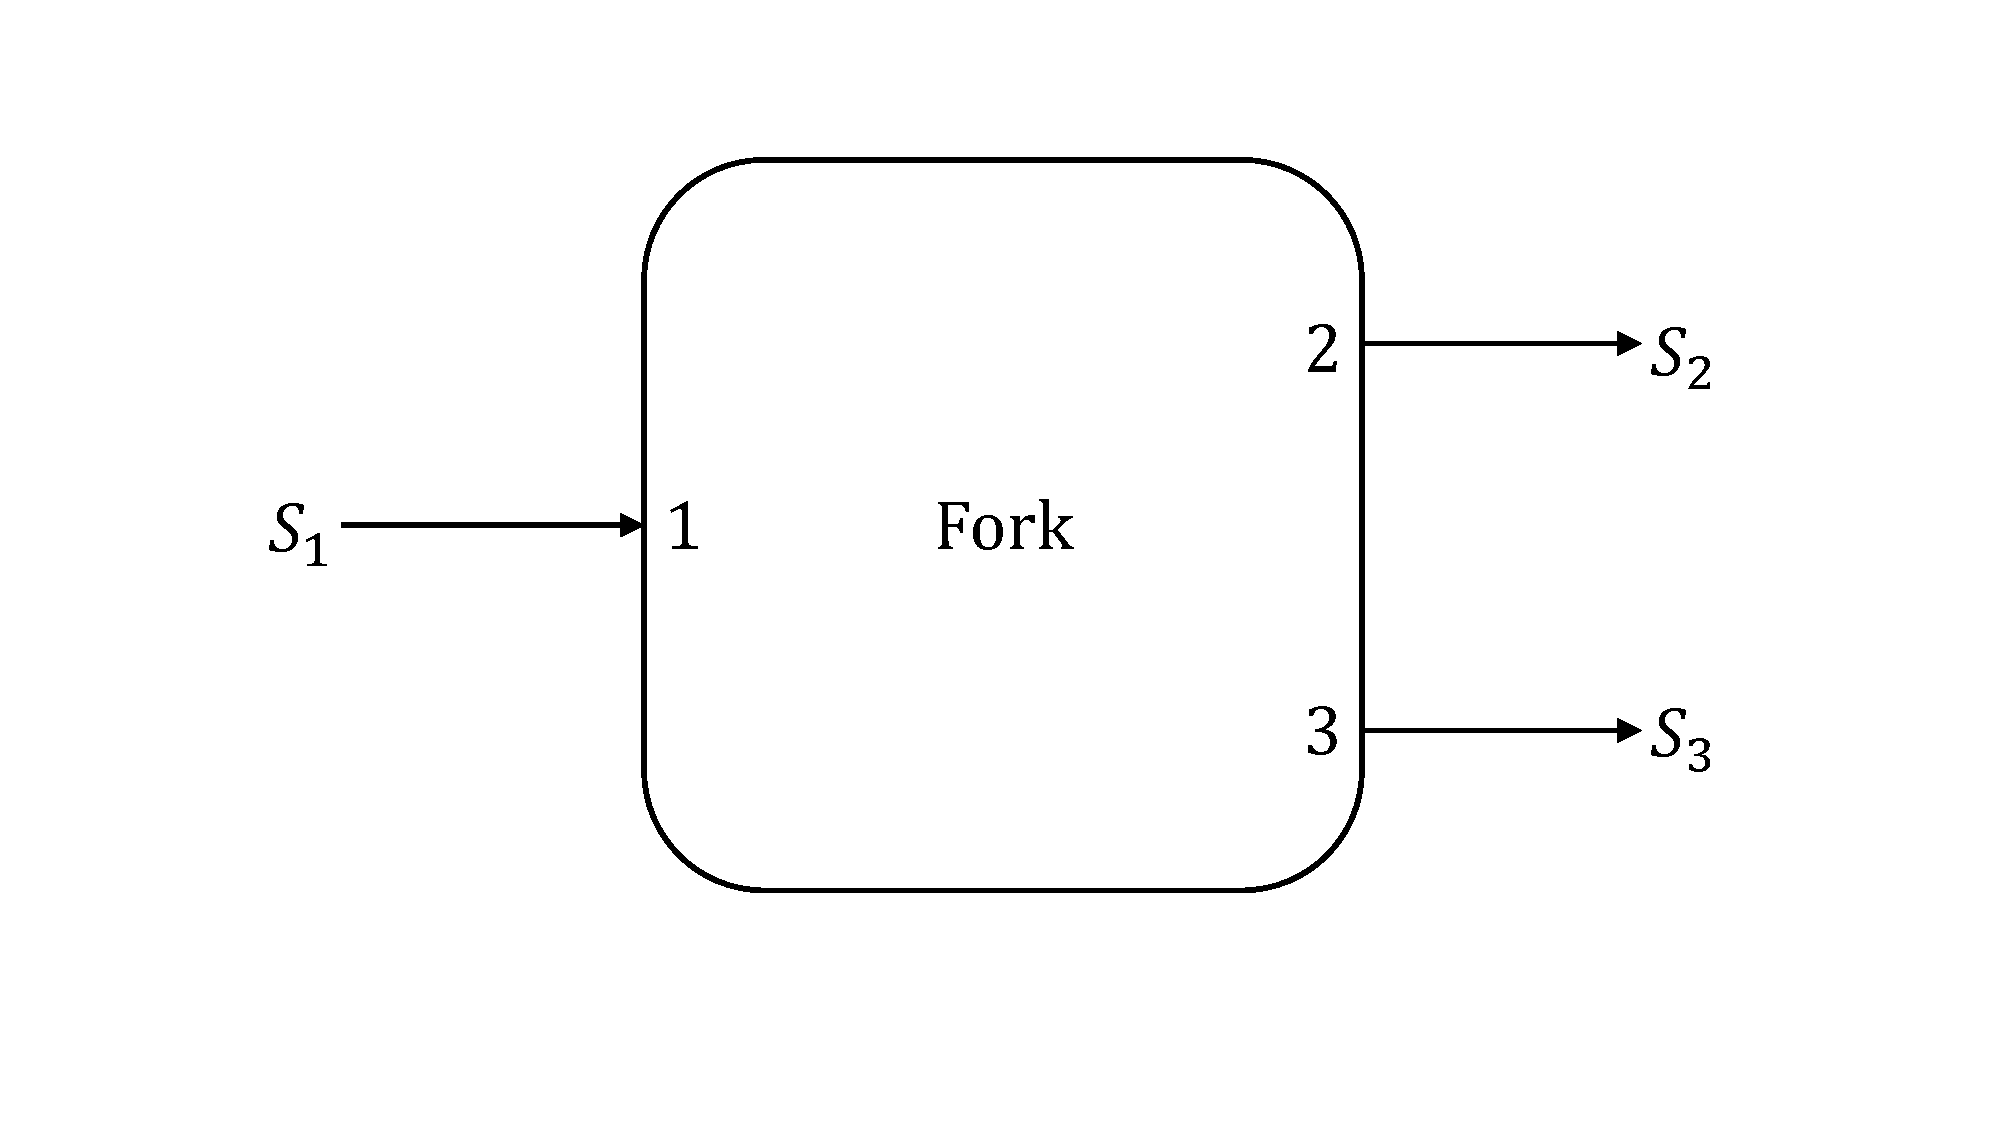
\includegraphics[width=1.0\textwidth, height=8cm]{./lib/fork/figures/fork.pdf}
	\caption{Fork}\label{}
\end{figure}